\documentclass{beamer}
\mode<presentation>
{
  \usetheme{Warsaw}
  \definecolor{mcgarnet}{rgb}{0.38, 0, 0.08}
  \definecolor{mcgray}{rgb}{0.6, 0.6, 0.6}
  \setbeamercolor{structure}{fg=mcgarnet,bg=mcgray}
  %\setbeamercovered{transparent}
}


\usepackage[english]{babel}
\usepackage[latin1]{inputenc}
\usepackage{times}
\usepackage[T1]{fontenc}
\usepackage{tikz}
\usepackage{graphicx}

\newcommand{\imagesource}[1]{{\centering\hfill\break\hbox{\scriptsize Image Source:\thinspace{\small\itshape #1}}\par}}

\title{A Glimpse of Data Structures}


\author{Robert Lowe\\}

\institute[Maryville College] % (optional, but mostly needed)
{
  Division of Mathematics and Computer Science\\
  Maryville College
}

\date[]{}
\subject{}

\pgfdeclareimage[height=0.5cm]{university-logo}{images/Maryville-College}
\logo{\pgfuseimage{university-logo}}



\AtBeginSection[]
{
  \begin{frame}<beamer>{Outline}
    \tableofcontents[currentsection]
  \end{frame}
}


\begin{document}

\begin{frame}
  \titlepage
\end{frame}

\begin{frame}{Outline}
  \tableofcontents
\end{frame}


% Structuring a talk is a difficult task and the following structure
% may not be suitable. Here are some rules that apply for this
% solution: 

% - Exactly two or three sections (other than the summary).
% - At *most* three subsections per section.
% - Talk about 30s to 2min per frame. So there should be between about
%   15 and 30 frames, all told.

% - A conference audience is likely to know very little of what you
%   are going to talk about. So *simplify*!
% - In a 20min talk, getting the main ideas across is hard
%   enough. Leave out details, even if it means being less precise than
%   you think necessary.
% - If you omit details that are vital to the proof/implementation,
%   just say so once. Everybody will be happy with that.
\section{Overview of Data Structures}

\begin{frame}{What are data structures?}
    \begin{columns}
        \column{0.5\textwidth}
        \begin{itemize}[<+->]
            \item Data structures are methods of organizing data in memory.
            \item Typically pieced together using pointers.
            \item Usually have some sort of mathematical property to them.
        \end{itemize}
        \column{0.5\textwidth}
        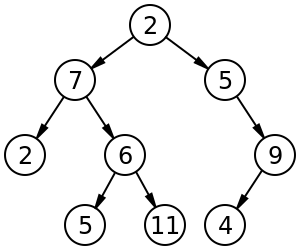
\includegraphics[width=\textwidth]{images/Binary_tree}
        \imagesource{wikipedia.org}
    \end{columns}
\end{frame}

\begin{frame}{Why do we need data structures?}
    \begin{columns}
        \column{0.5\textwidth}
        \begin{itemize}[<+->]
            \item Good memory organization leads to good algorithms.
            \item Semantic information can be folded into the structure of memory.
            \item We can reduce search times, process complex input, and solve otherwise difficult problems with data structures.
            
            \item For example, compilers are based on trees!
        \end{itemize}
        \column{0.5\textwidth}
        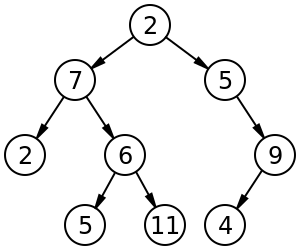
\includegraphics[width=\textwidth]{images/Binary_tree}
        \imagesource{wikipedia.org}
    \end{columns}
\end{frame}

\begin{frame}{Some Standard Data Structures}
    \begin{description}[<+->]
    \item[Linked List] A simple sequential container where every node contains a link to the next node.
    \item[Stack] A list where we always insert and remove from the head.
    \item[Queue] A list where we always insert at the tail and remove from the head.
    \item[Tree] A recursive structure where each node has links to two or more nodes.
    \item[Binary Tree] A tree where each node has a maximum of two children.
    \item[Heap] A tree which satisfies the heap property.
    \item[Search Tree] A tree with some sort of ordering imposed on the nodes.
    \item[Red-Black Tree] A self-balancing binary search tree.
    \end{description}
\end{frame}

\section{Linked Lists}
\begin{frame}{Linked Lists}
    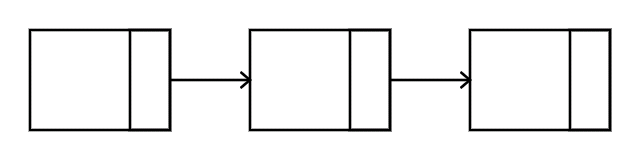
\includegraphics[height=0.25\textheight]{images/LinkedList}
    \begin{itemize}[<+->]
        \item A sequential container.
        \item Each node contains a data field and a pointer to the next node.
        \item Nodes can be located anywhere in memory.
        \item Insertion and deletion are handled by manipulating the links.
    \end{itemize}
\end{frame}

\begin{frame}[fragile]{The Node Structure}
    \begin{verbatim}
struct ListNode {
    int data;
    ListNode *next;
};
    \end{verbatim}
    \begin{itemize}[<+->]
        \item Here we have a node which can store an integer.
        \item Structure is provided by the {\tt next} pointer.
        \item It is more typical in C++ to use templates for data structures, but here we will use integers to simplify the discussion. 
    \end{itemize}
\end{frame}

\begin{frame}{Basic List Operations}
   \begin{description}[<+->]
       \item[insert] Place an element at a specified location in the list.
       \item[remove] Remove a node from the list.
       \item[append] Insert an element at the tail (end) of the list.
       \item[prepend] Insert an element at the head (beginning) of the list.
   \end{description}
\end{frame}

\begin{frame}{Insert}
   \begin{enumerate}[<+->]
       \item Create the new node.
           \par 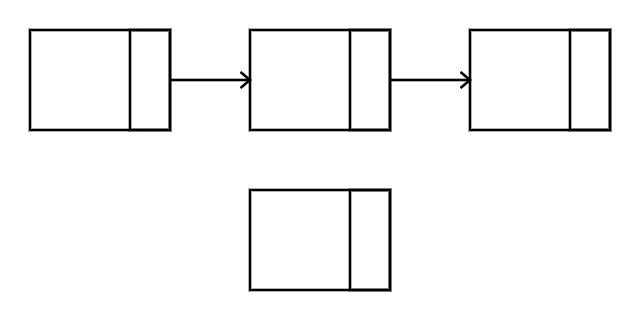
\includegraphics[height=0.20\textheight]{images/Linking1}
       \item Set the new node's next to the previous node's next.
           \par 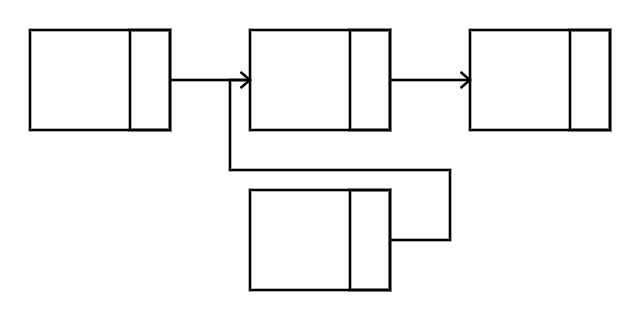
\includegraphics[height=0.20\textheight]{images/Linking2}
       \item Set the previous node's next to the new node.
           \par 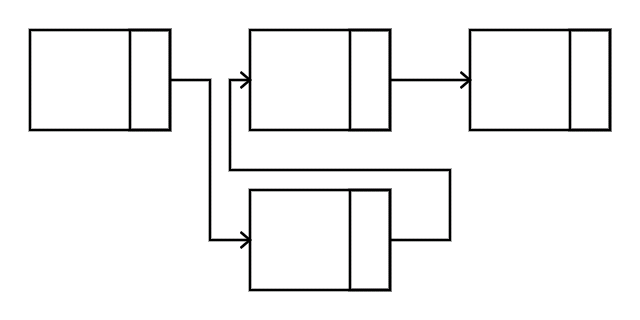
\includegraphics[height=0.20\textheight]{images/Linking3}
   \end{enumerate}
\end{frame}


\begin{frame}{Remove}
    \begin{enumerate}[<+->]
    \item Find the previous node.
    \item Unlink the node from the list.
        \par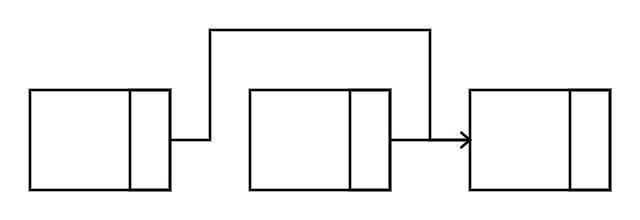
\includegraphics[height=0.25\textheight]{images/Removing1}
    \item Delete the node.
        \par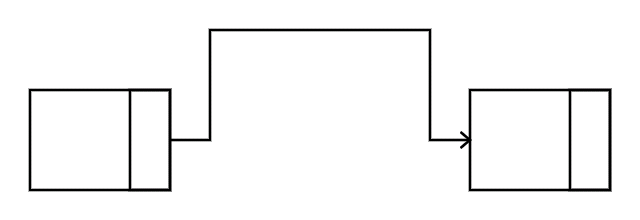
\includegraphics[height=0.25\textheight]{images/Removing2}
    \end{enumerate}
\end{frame}

\begin{frame}[fragile]{Traversing a Linked List}
    \begin{verbatim}
for(ListNode *cur = head;  cur != nullptr; 
    cur = cur->next) {
  cout << cur->data << endl;
}
    \end{verbatim}
    \begin{itemize}[<+->]
        \item A linked list is "traversed" by visiting each of its nodes in turn.
        \item This is accomplished by following all of its "next" pointers.
    \end{itemize}
\end{frame}

\begin{frame}{When to Use a Linked List}
    \begin{itemize}[<+->]
        \item Linked Lists are best used when sequential storage is needed.
        \item As linked lists cannot be accessed randomly, they are a poor choice for dynamic arrays (like vectors).
        \item Example: The C call stack uses a linked-list structure for its stack frames.
        \item Stacks and Queues work well as linked list implementations.
    \end{itemize}
\end{frame}

\end{document}


